\section{Historical Evolution and Related Work}
\label{sec:history_and_related_work}

The design of artificial memory systems has evolved through seventeen distinct stages over more than five decades, progressing from symbolic production rules to version-controlled cognitive DAGs. Fig.~\ref{fig:history_timeline} summarizes this evolutionary trajectory.

\begin{figure*}[t]
\centering
\resizebox{0.95\textwidth}{!}{%
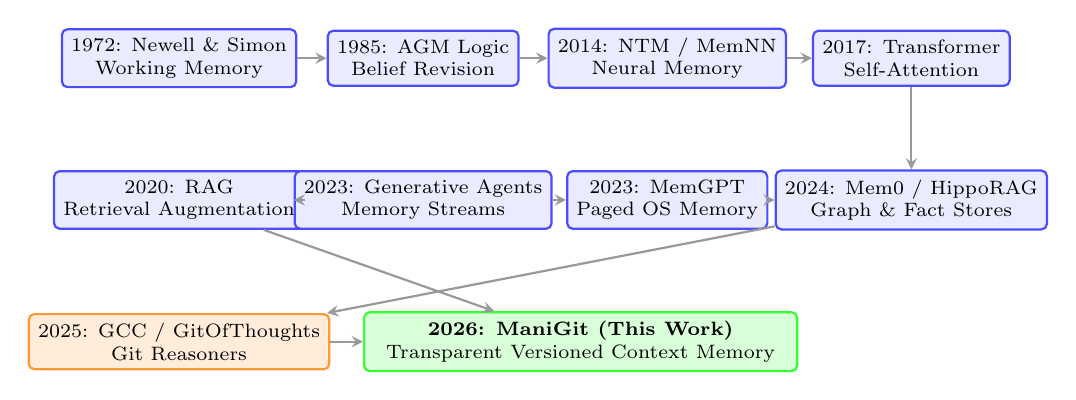
\begin{tikzpicture}[node distance=1.3cm, auto,
    every node/.style={font=\scriptsize},
    stage/.style={rectangle, draw=blue!70, fill=blue!8, thick, minimum width=2.4cm, minimum height=0.7cm, align=center, rounded corners=2pt},
    arrow/.style={->, >=stealth, thick, color=gray!80}]

\node[stage] (s1) {1972: Newell \& Simon\\Working Memory};
\node[stage, right of=s1, xshift=1.8cm] (s2) {1985: AGM Logic\\Belief Revision};
\node[stage, right of=s2, xshift=1.8cm] (s3) {2014: NTM / MemNN\\Neural Memory};
\node[stage, right of=s3, xshift=1.8cm] (s4) {2017: Transformer\\Self-Attention};

\node[stage, below of=s1, yshift=-0.5cm] (s5) {2020: RAG\\Retrieval Augmentation};
\node[stage, right of=s5, xshift=1.8cm] (s6) {2023: Generative Agents\\Memory Streams};
\node[stage, right of=s6, xshift=1.8cm] (s7) {2023: MemGPT\\Paged OS Memory};
\node[stage, right of=s7, xshift=1.8cm] (s8) {2024: Mem0 / HippoRAG\\Graph \& Fact Stores};

\node[stage, below of=s5, yshift=-0.5cm, fill=orange!15, draw=orange!80] (s9) {2025: GCC / GitOfThoughts\\Git Reasoners};
\node[stage, right of=s9, xshift=3.8cm, fill=green!15, draw=green!80, minimum width=5.5cm] (s10) {\textbf{2026: ManiGit (This Work)}\\Transparent Versioned Context Memory};

\draw[arrow] (s1) -- (s2);
\draw[arrow] (s2) -- (s3);
\draw[arrow] (s3) -- (s4);
\draw[arrow] (s4) -- (s8);
\draw[arrow] (s5) -- (s6);
\draw[arrow] (s6) -- (s7);
\draw[arrow] (s7) -- (s8);
\draw[arrow] (s8) -- (s9);
\draw[arrow] (s9) -- (s10);
\draw[arrow] (s5) -- (s10);

\end{tikzpicture}%
}

\caption{Historical evolution of agent memory architectures from classical AI production systems (1972) and formal belief revision (1985) to differentiable neural memory, retrieval-augmented generation, operating-system-inspired paging, and transparent versioned context memory.}
\label{fig:history_timeline}
\end{figure*}

\subsection{Foundations: Production Rules and Belief Revision}
The conceptual separation between bounded working memory and persistent long-term knowledge traces back to Newell and Simon's seminal work on human problem solving~\cite{newell1972human}. Production systems formalized memory as an active working memory buffer holding immediate goal chunks, interacting with a persistent repository of declarative rules. However, classical production systems relied on manual symbolic engineering and lacked natural language adaptability.

Concurrently, the philosophical and mathematical foundations of memory updating were established by Alchourr{\'o}n, G{\"a}rdenfors, and Makinson~\cite{agm1985logic} in the AGM belief revision framework. AGM formalized the logical postulates of \textit{Success} (incorporating new facts), \textit{Consistency} (avoiding contradictory states), and \textit{Minimal Change} (minimizing information loss during contraction). While theoretically rigorous, classical belief revision was computationally intractable for open-domain natural language and modeled belief contraction destructively, erasing retracted propositions from active consideration.

\subsection{Differentiable Neural Memory}
In the deep learning era, researchers attempted to augment recurrent neural networks with external continuous memory arrays. Graves et al.~\cite{graves2014neural} introduced \textit{Neural Turing Machines} (NTM), enabling networks to read and write to continuous memory matrices via differentiable addressing. Weston et al.~\cite{weston2014memory} proposed \textit{Memory Networks}, using continuous memory slot arrays to execute multi-hop reasoning over synthetic question-answering tasks. Graves et al.~\cite{graves2016hybrid} advanced this with the \textit{Differentiable Neural Computer} (DNC), incorporating a temporal link matrix to track the chronological sequence of memory allocations. While foundational, differentiable neural computers proved notoriously difficult to optimize and could not scale to open-domain natural language dialogues.

\subsection{RAG and Conversational Buffers}
The rise of large pre-trained language models shifted the memory paradigm toward non-parametric retrieval. REALM~\cite{guu2020realm} and RAG~\cite{lewis2020retrieval} established dense passage retrieval as the dominant mechanism for externalizing knowledge without fine-tuning model parameters. In conversational settings, early assistant implementations introduced sliding conversation buffers and running summaries. However, as demonstrated in our experiments, sliding windows drop foundational instructions when dialogue exceeds buffer length, while running summaries irreversibly discard exact technical constraints through lossy paraphrase.

\subsection{Modern Persistent Agent Memory Systems}
Over the past three years, persistent agent memory has become an active frontier:
\begin{itemize}
    \item \textbf{Cognitive and Reflection Streams:} Park et al.~\cite{park2023generative} demonstrated that simulated agents could maintain multi-day social relationships using an append-only memory stream scored by recency, importance, and relevance, paired with periodic synthetic reflection. Zhong et al.~\cite{zhong2023memorybank} introduced \textit{MemoryBank}, applying an exponential Ebbinghaus forgetting curve to prioritize recently reinforced memories.
    \item \textbf{Operating-System Architectures:} Packer et al.~\cite{packer2023memgpt} introduced \textit{MemGPT}, treating the context window as RAM and external databases as disk, managed through explicit LLM tool calls. Kang et al.~\cite{kang2025memoryos} formalized operating-system-inspired memory hierarchies for LLM agents, structuring memory across short-term, mid-term, and persistent tiers.
    \item \textbf{Graph and Networked Memory:} Guti{\'e}rrez et al.~\cite{gutierrez2024hipporag} developed \textit{HippoRAG}, mimicking mammalian hippocampal indexing via Personalized PageRank over knowledge graphs. Edge et al.~\cite{edge2024graphrag} introduced \textit{Graph RAG}, using graph community detection for hierarchical corpus summarization. Xu et al.~\cite{xu2024amem} proposed \textit{A-MEM}, structuring memories into Zettelkasten-style interconnected note networks.
    \item \textbf{Commercial Fact Stores:} Deshmukh et al.~\cite{deshmukh2024mem0} developed \textit{Mem0}, providing a multi-scope memory orchestration layer (user, session, agent) with hybrid vector-graph backends.
\end{itemize}

\subsection{Emergence of Git Metaphors in Agent State}
Most recently, researchers have explored applying Git-like version control metaphors to LLM agents:
\begin{itemize}
    \item \textbf{Git Context Controller (GCC):} Wu et al.~\cite{wu2025gcc} proposed GCC, equipping software engineering agents on SWE-bench with explicit commands (\texttt{COMMIT}, \texttt{BRANCH}, \texttt{MERGE}, \texttt{CONTEXT}) to manage Markdown notes in a local workspace directory.
    \item \textbf{GitOfThoughts:} Shekar et al.~\cite{shekar2025gitofthoughts} introduced GitOfThoughts, mapping tree-of-thoughts reasoning paths into native Git commits for mathematical problem solving.
\end{itemize}

As analyzed in Section~\ref{sec:research_gap}, while GCC and GitOfThoughts validate the conceptual appeal of Git for agent workflows, both systems require the agent to manually execute version-control tool calls, lack automated memory intake classification, do not maintain functional memory tiers, and lack budget-constrained knapsack context compilation.
